\section{Results}
\label{cost-benefit:results}

This section presents the results of applying the methodology discussed in
Section~\ref{cost-benefit:methodology} to \FFWithVersion.  The section first
describes each \WAS~'s benefit, and follows with each standard's cost.

\begin{table}[ht]
  \captionsetup{font=footnotesize,singlelinecheck=off}
  \centering
  %   \rowcolors{2}{gray!25}{white}
  \resizebox{\textwidth}{!}{
  \begin{tabular}{ l | l r r r | r r | r | l }
    \toprule
      Standard Name                                     & Abbreviation & \#
    \ATK & Site Break & Agree & \# CVEs & \# High or & \% ELoC & Enabled \\
                                                        &              & Using
      & Rate & \% & & Severe & & attacks \\
    \midrule
      WebGL                                               &  WEBGL       & 852   & \textless1\% & 93\%  & 31  & 22 & 27.43 & \cite{laperdrix2016beauty,alaca2016device,ho2014tick,cao2017cross} \\ % 20751 \\
      HTML: Web Workers                                   &  H-WW        & 856   & 0\%          & 100\% & 16  & 9  & 1.63  & \cite{ho2014tick,gras2017aslr} \\ % 1238 \\
      WebRTC                                              &  WRTC        & 24    & 0\%          & 93\%  & 15  & 4  & 2.48  & \cite{englehardt2016online,alaca2016device} \\ % 1878 \\
      HTML: The canvas element                            &  H-C         & 6935  & 0\%          & 100\% & 14  & 6  & 5.03  & \cite{englehardt2016online,laperdrix2016beauty,alaca2016device,acar2014web,kotcher2013cross,ho2014tick,cao2017cross} \\ % 3810 \\
      Scalable Vector Graphics                            &  SVG         & 1516  & 0\%          & 98\%  & 13  & 10 & 7.86  & \\ % 5949 \\
      Web Audio API                                       &  WEBA        & 148   & 0\%          & 100\% & 10  & 5  & 5.79  & \cite{englehardt2016online,alaca2016device} \\ % 4380 \\
      XMLHttpRequest                                      &  AJAX        & 7806  & 32\%         & 82\%  & 11  & 4  & 1.73  & \\ % 1312 \\
      HTML                                                &  HTML        & 8939  & 40\%         & 85\%  & 6   & 2  & 0.89  & \cite{nikiforakis2013cookieless,acar2013fpdetective} \\ % 677 \\
      HTML 5                                              &  HTML5       & 6882  & 4\%          & 97\%  & 5   & 2  & 5.72  & \\ % 4332 \\
      Service Workers                                     &  SW          & 0     & 0\%          & -     & 5   & 0  & 2.84  & \cite{van2016request,gelernter2015cross,van2015clock} \\ % 2150 \\
      HTML: Web Sockets                                   &  H-WS        & 514   & 0\%          & 95\%  & 5   & 3  & 0.67  & \\ % 508 \\
      HTML: History Interface                             &  H-HI        & 1481  & 1\%          & 96\%  & 5   & 1  & 1.04  & \\ % 790 \\
      Indexed Database API                                &  IDB         & 288   & \textless1\% & 100\% & 4   & 2  & 4.73  & \cite{alaca2016device,acar2014web} \\ % 3583 \\
      Web Cryptography API                                &  WCR         & 7048  & 4\%          & 90\%  & 4   & 3  & 0.52  & \\ % 400 \\
      Media Capture and Streams                           &  MCS         & 49    & 0\%          & 95\%  & 4   & 3  & 1.08  & \cite{tian2014all} \\ % 819 \\
      DOM Level 2: HTML                                   &  DOM2-H      & 8956  & 13\%         & 89\%  & 3   & 1  & 2.09  & \\ % 1588 \\
      DOM Level 2: Traversal and Range                    &  DOM2-T      & 4406  & 0\%          & 100\% & 3   & 2  & 0.04  & \\ % 32 \\
      HTML 5.1                                            &  HTML51      & 2     & 0\%          & 100\% & 3   & 1  & 1.18  & \\ % 895 \\
      Resource Timing                                     &  RT          & 433   & 0\%          & 98\%  & 3   & 0  & 0.10  & \\ % 81 \\
      Fullscreen API                                      &  FULL        & 229   & 0\%          & 95\%  & 3   & 1  & 0.12  & \\ % 96 \\
      Beacon                                              &  BE          & 2302  & 0\%          & 100\% & 2   & 0  & 0.23  & \\ % 175 \\
      DOM Level 1                                         &  DOM1        & 9113  & 63\%         & 96\%  & 2   & 2  & 1.66  & \\ % 1258 \\
      DOM Parsing and Serialization                       &  DOM-PS      & 2814  & 0\%          & 83\%  & 2   & 1  & 0.31  & \\ % 235 \\
      DOM Level 2: Events                                 &  DOM2-E      & 9038  & 34\%         & 96\%  & 2   & 0  & 0.35  & \\ % 270 \\
      DOM Level 2: Style                                  &  DOM2-S      & 8773  & 31\%         & 93\%  & 2   & 1  & 0.69  & \\ % 523 \\
      Fetch                                               &  F           & 63    & \textless1\% & 90\%  & 2   & 0  & 1.14  & \cite{van2016request,gelernter2015cross,van2015clock} \\ % 869 \\
      CSS Object Model                                    &  CSS-OM      & 8094  & 5\%          & 94\%  & 1   & 0  & 0.17  & \cite{nikiforakis2013cookieless} \\ % 131 \\
      DOM                                                 &  DOM         & 9050  & 36\%         & 94\%  & 1   & 1  & 1.29  & \\ % 983 \\
      HTML: Plugins                                       &  H-P         & 92    & 0\%          & 100\% & 1   & 1  & 0.98  & \cite{alaca2016device,acar2013fpdetective} \\ % 743 \\
      File API                                            &  FA          & 1672  & 0\%          & 83\%  & 1   & 0  & 1.46  & \\ % 1110 \\
      Gamepad                                             &  GP          & 1     & 0\%          & 71\%  & 1   & 1  & 0.07  & \\ % 60 \\
      Geolocation API                                     &  GEO         & 153   & 0\%          & 96\%  & 1   & 0  & 0.26  & \cite{xu2015ucognito,kim2014exploring} \\ % 198 \\
      High Resolution Time Level 2                        &  HRT         & 5665  & 0\%          & 100\% & 1   & 0  & 0.02  & \cite{gelernter2015cross,andrysco2015subnormal,oren2015spy,van2015clock,kotcher2013cross,ho2014tick,gruss2015practical,gras2017aslr} \\ % 22 \\
      HTML: Channel Messaging                             &  H-CM        & 4964  & 0\%          & 0.025 & 1   & 0  & 0.40  & \cite{weissbacher2015zigzag,son2013postman} \\ % 309 \\
      Navigation Timing                                   &  NT          & 64    & 0\%          & 98\%  & 1   & 0  & 0.09  & \\ % 75 \\
      Web Notifications                                   &  WN          & 15    & 0\%          & 100\% & 1   & 1  & 0.82  & \\ % 622 \\
      Page Visibility (Second Edition)                    &  PV          & 0     & 0\%          & -     & 1   & 1  & 0.02  & \\ % 20 \\
      UI Events                                           &  UIE         & 1030  & \textless1\% & 100\% & 1   & 0  & 0.47  & \\ % 362 \\
      Vibration API                                       &  V           & 1     & 0\%          & 100\% & 1   & 1  & 0.08  & \\ % 67 \\
      Console API                                         &  CO          & 3     & 0\%          & 100\% & 0   & 0  & 0.59  & \cite{ho2014tick} \\ % 452 \\
      CSSOM View Module                                   &  CSS-VM      & 4538  & 0\%          & 100\% & 0   & 0  & 2.85  & \cite{acar2013fpdetective} \\ % 2159 \\
      Battery Status API                                  &  BA          & 2317  & 0\%          & 100\% & 0   & 0  & 0.15  & \cite{englehardt2016online,alaca2016device,nikiforakis2013cookieless,olejnik2015leaking} \\ % 120 \\
      CSS Conditional Rules Module Lvl 3                &  CSS-CR      & 416   & 0\%          & 100\% & 0   & 0  & 0.16  & \\ % 126 \\
      CSS Font Loading Module Level 3                     &  CSS-FO      & 2287  & 0\%          & 98\%  & 0   & 0  & 1.24  & \cite{alaca2016device,acar2013fpdetective} \\ % 942 \\
      DeviceOrientation Event                             &  DO          & 0     & 0\%          & -     & 0   & 0  & 0.06  & \cite{das2016tracking,alaca2016device} \\ % 48 \\
      % Directory Upload                                    &  DU          & 0     & 0\%          & -     & 0   & 0  & 0.94  & \\ % 714 \\
      DOM Level 2: Core                                   &  DOM2-C      & 8896  & 89\%         & 97\%  & 0   & 0  & 0.29  & \\ % 225 \\
      DOM Level 3: Core                                   &  DOM3-C      & 8411  & 4\%          & 96\%  & 0   & 0  & 0.25  & \\ % 194 \\
      DOM Level 3: XPath                                  &  DOM3-X      & 364   & 1\%          & 97\%  & 0   & 0  & 0.16  & \\ % 126 \\
      % Encoding                                            &  E           & 1     & 0\%          & 100\% & 0   & 0  & 0.21  & \\ % 165 \\
      Encrypted Media Extensions                          &  EME         & 9     & 0\%          & 100\% & 0   & 0  & 1.91  & \\ % 1449 \\
      % execCommand                                         &  EC          & 2419  & 0\%          & 100\% & 0   & 0  & 0.00  & \\ % 0 \\
      % Geometry Interfaces Module Level 1                  &  GIM         & 0     & 0\%          & -     & 0   & 0  & 0.71  & \\ % 538 \\
      % HTML: Broadcasting                                  &  H-B         & 1     & 0\%          & 100\% & 0   & 0  & 0.26  & \\ % 204 \\
      HTML: Web Storage                                   &  H-WB        & 7806  & 0\%          & 83\%  & 0   & 0  & 0.55  & \cite{alaca2016device,xu2015ucognito,ho2014tick} \\ % 421 \\
      % HTML Editing APIs                                   &  H-E         & 0     & 0\%          & -     & 0   & 0  & 0.00  & \\ % 0 \\
      % Media Capture from DOM Elements                     &  MCD         & 0     & 0\%          & -     & 0   & 0  & 0.28  & \\ % 212 \\
      Media Source Extensions                             &  MSE         & 1240  & 0\%          & 95\%  & 0   & 0  & 1.97  & \\ % 1495 \\
      % MediaStream Recording                               &  MSR         & 0     & 0\%          & -     & 0   & 0  & 0.55  & \\ % 417 \\
      % Performance Timeline                                &  PT          & 4535  & 0\%          & 95\%  & 0   & 0  & 0.04  & \\ % 32 \\
      % Performance Timeline Level 2                        &  PT2         & 1672  & 0\%          & 98\%  & 0   & 0  & 0.21  & \\ % 159 \\
      % Pointer Lock                                        &  PL          & 18    & 0\%          & 100\% & 0   & 0  & 0.03  & \\ % 29 \\
      % Proximity Events                                    &  PE          & 18    & 0\%          & 100\% & 0   & 0  & 0.01  & \\ % 8 \\
      % Selection API                                       &  SEL         & 2287  & 0\%          & 100\% & 0   & 0  & 0.02  & \\ % 22 \\
      Selectors API Level 1                               &  SLC         & 8611  & 15\%         & 89\%  & 0   & 0  & 0.00  & \\ % 0 \\
      % Shadow DOM                                          &  SD          & 0     & 0\%          & -     & 0   & 0  & 0.34  & \\ % 261 \\
      % The Screen Orientation API                          &  SO          & 38    & 0\%          & 100\% & 0   & 0  & 0.34  & \\ % 261 \\
      Script-based animation timing control          &  TC          & 3437  & 0\%          & 100\% & 0   & 0  & 0.08  & \cite{nikiforakis2013cookieless} \\ % 67 \\
      % Tracking Preference Expression                      &  TPE         & 0     & 0\%          & -     & 0   & 0  & 0.01  & \\ % 10 \\
      % URL                                                 &  URL         & 5     & 0\%          & 100\% & 0   & 0  & 0.59  & \\ % 453 \\
      % User Timing Level 2                                 &  UTL         & 3077  & 0\%          & 100\% & 0   & 0  & 0.44  & \\ % 340 \\
      % W3C DOM4                                            &  DOM4        & 5639  & 0\%          & 100\% & 0   & 0  & 0.45  & \\ % 346 \\
      % WebVTT                                              &  WEBVTT      & 0     & 0\%          & -     & 0   & 0  & 0.44  & \\ % 334 \\
      Ambient Light Sensor API                            &  ALS         & 18    & 0\%          & 89\%  & 0   & 0  & 0.00  & \cite{nikiforakis2013cookieless,olejnik2017stealing} \\ % 0 \\
    \bottomrule
  \end{tabular}
  }
  \caption{
    Data on all \NumStandards measured \WASs, excluding 20 standards with a 0\% break rate, 0 associated CVEs
    and accounting for less than one percent of measured effective lines of code.
  }
  \begin{small}
    \begin{itemize}
      \setlength{\itemsep}{-2pt}
      \item The standard's full name
      \item The abbreviation used when referencing this standard in this work
      \item The number of sites in the Alexa 10k using the standard (Section~\ref{measuement:results})
      \item The portion of measured sites that were broken by disabling the
        standard. (Section~\ref{cost-benefit:methodology:per-standard-benefit})
      \item The agreement between testers' evaluation (Section~\ref{cost-benefit:methodology:per-standard-benefit})
      \item The number of CVEs since 2010 associated with the feature (Section~\ref{cost-benefit:results:costs-cves})
      \item The number of CVEs since 2010 ranked as ``high'' or ``severe'' (Section~\ref{cost-benefit:results:costs-cves})
      \item The percentage of \gls{eloc} for this
        standard, as a percentage of all attributed lines (Section~\ref{cost-benefit:methodology:costs-loc})
      \item Citations for papers describing attacks relying on the standard (Section~\ref{cost-benefit:results:costs-research})
    \end{itemize}
  \end{small}
  \label{table:megatable}
\end{table}



\subsection{Per-Standard Benefit}
\label{cost-benefit:results:results-benefit}
\begin{figure}[ht]
  \centering
  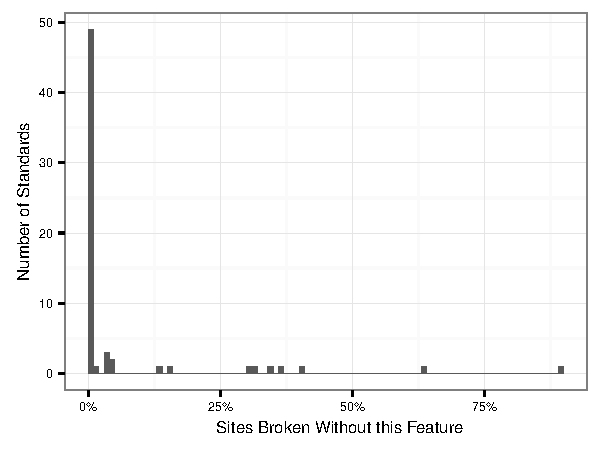
\includegraphics[width=.5\textwidth]{figures/breakrate_histogram.pdf}
  \caption{A histogram giving the number of standards binned by the percentage of sites that broke when removing the standard.}
  \label{fig:feature-benefit}
\end{figure}

As explained in Section~\ref{cost-benefit:methodology:per-standard-benefit},
our workers conducted up to \NumSitesPerStandard measurements of websites in
the \ATK known to use each \WAS. If a standard was observed being used
fewer than \NumSitesPerStandard times within the \ATK, all sites using that
standard were measured. In total, we did two measurements of 1,684 (website,
disabled feature) tuples, one by each worker.

\ref{fig:feature-benefit} gives a histogram of the break rates for each of
the \NumStandards standards measured in this work.  As the graph shows, removing
over 60\% of the measured standards resulted in no noticeable effect on the
user's experience.

In some cases, this was because the standard was never observed being
used\footnote{e.g. The \textit{WebVTT} standard, which allows document authors
to synchronize text changes with media playing on the page.}.  In other cases,
it was because the standard is intended to be used in a way that users do not
notice\footnote{e.g. The \textit{Beacon} standard, which allows content authors
to trigger code execution when a user browses away from a website.}.

Other standards caused a large number of sites to break when removed from the
browser.  Disabling access to the \textit{DOM 1} standard (which provides basic
functionality for modifying the text and appearance of a document) broke an
estimated 69.05\% of the web.

A listing of the site break rate for all \NumStandards standards is provided
in \ref{table:megatable}.

For emphasis, we note again that these measurements only cover interacting with
websites as an anonymous, unauthenticated user. It is possible that site
feature use changes when users log into websites, since some sites only provide
full functionality to registered users.


\subsection{Per-Standard Cost}
\label{cost-benefit:results:results-costs}
As described in Section~\ref{cost-benefit:methodology:per-standard-cost}, we
measured the cost of a \WAS being available in the browser in three ways: first
as the number of times the standard is leveraged by attacks in high quality
peer-reviewed research (Section~\ref{cost-benefit:results:costs-research}),
second as the number of \gls{cve}s reported against the standard between 2010
and 2015 (Section~\ref{cost-benefit:results:costs-cves}), and third with a
lower bound estimate of the number of \gls{eloc} needed to implement the
standard in the browser (Section~\ref{cost-benefit:results:costs-loc}).


\subsubsection{Attacks from Related Research}
\label{cost-benefit:results:costs-research}
We searched the work published at major research conferences and journals
between 2010 and 2015 for research on browser weaknesses related to \WASs.
These papers either explicitly identified either a \WAS, or a feature or
functionality uniquely related to a \WAS.  In each case the standard was either
necessary for the documented attack to succeed, or was used to make the attack
faster or more reliable.  Since academic attacks emphasize attack novelty,
instead of only finding all existing vulnerabilities, the use of a \WAS in
academic literature suggests that the \WAS allowed new browser exploits.

The most frequently cited standard was the \textit{High Resolution Time Level
2}~\cite{highres2016w3c} standard, which provides highly accurate,
millisecond-resolution timers.  Seven papers published since 2013 leverage the
standard to break the isolation protections provided by the browser, such as
learning information about the environment the browser is running
in~\cite{ho2014tick,oren2015spy,gruss2015practical}, learning information about
other open browser
windows~\cite{andrysco2015subnormal,kotcher2013cross,gruss2015practical}, and
gaining identifying information from other domains~\cite{van2015clock}.

Other implicated standards include the \textit{Canvas} standard, which was
identified by researchers as allowing attackers to persistently track users
across websites~\cite{acar2014web}, learn about the browser's execution
environment~\cite{ho2014tick} or obtain information from other browsing
windows~\cite{kotcher2013cross}, and the \textit{Media Capture and Streams}
standard, which was used by researchers to perform ``cross-site request
forgery, history sniffing, and information stealing''
attacks~\cite{tian2014all}.

In total we identified \NumAttackPapers papers leveraging \NumAttackStandards
standards to attack the privacy and security protections of the web browser.
Citations for these papers are included in \ref{table:megatable}.


\subsubsection{CVEs}
\label{cost-benefit:results:costs-cves}
\begin{figure}[th]
  \centering
  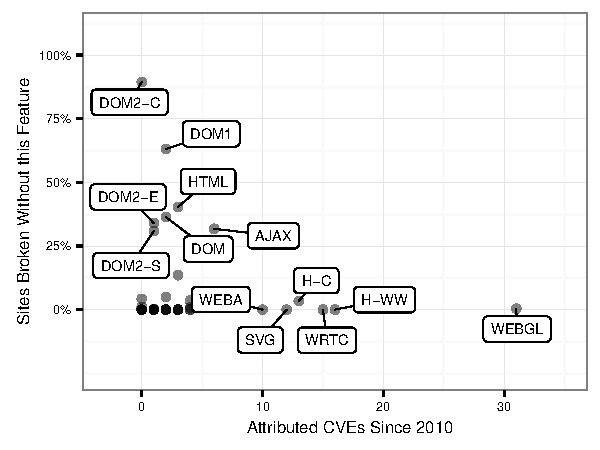
\includegraphics[width=.5\textwidth]{figures/cve_breakrate.pdf}
  \caption{A scatter plot showing the number of CVEs filed against each standard since 2010, by how many sites in the Alexa 10k break when the standard is removed.}
  \label{fig:cve-breakrate}
\end{figure}

\begin{figure}[t]
  \centering
  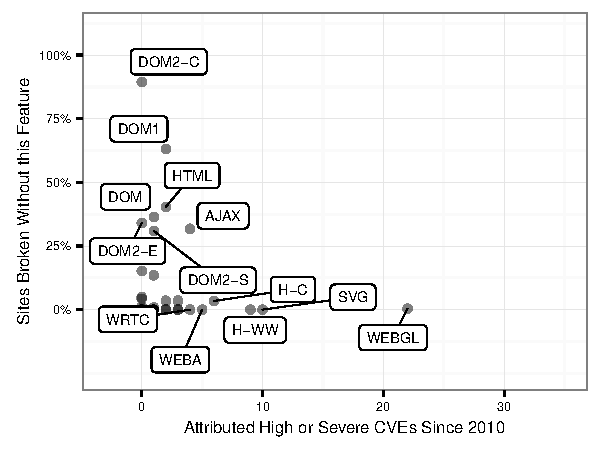
\includegraphics[width=.5\textwidth]{figures/cve_breakrate_severe.pdf}
  \caption{A scatter plot showing the number of ``high'' or ``severe'' CVEs filed against each standard since 2010, by how many sites in the Alexa 10k break when the standard is removed.}
  \label{fig:cve-breakrate-severe}
\end{figure}

Vulnerability reports are not evenly distributed across browser standards.
\ref{fig:cve-breakrate-severe} compares per-standard
benefit (measured by the number of sites that require the standard to function)
on the y-axis, against the number of severe \gls{cve}s associated with the
standard on the x-axis.  \ref{fig:cve-breakrate} shows a similar plot, but
includes all \gls{cve}s, not only high and severe ones.  Both figures
show the same general relationship between break rate and \gls{cve}s.

Points in the upper-left of each figure denote standards that are high benefit
and low cost  (i.e. standards that are frequently required on the web but have
rarely been implicated in \gls{cve}s).  For example, consider the
\textit{Document Object Model (DOM) Level 2 Events Specification} standard,
denoted by \textbf{DOM2-E} in \ref{fig:cve-breakrate-severe}.  This
standard allows website authors to trigger functionality to occur with
common browser events, like button clicks and mouse movement.  This standard is highly
beneficial to browser users, being required by 34\% of pages to function
correctly.  The standard entails little risk to web users, being
associated with zero \gls{cve}s since 2010.

Standards in the lower-right section of the figures, by contrast, bring
low benefit and high cost to users, when using \gls{cve} counts as a metric
for security cost.  For example, the \textit{WebGL} standard, denoted by
\textbf{WEBGL} in \ref{fig:cve-breakrate-severe}, allows websites to take
advantage of graphics hardware on the browsing device.
Less than 1\% of sites in the \ATK need the standard, but
the standard is implicated in 22 high or severe \gls{cve}s since 2010.  This
suggests that the standard poses a high security risk to users, with
little attenuating benefit.


\subsubsection{Implementation Complexity}
\label{cost-benefit:results:costs-loc}
\begin{figure}[ht]
  \centering
  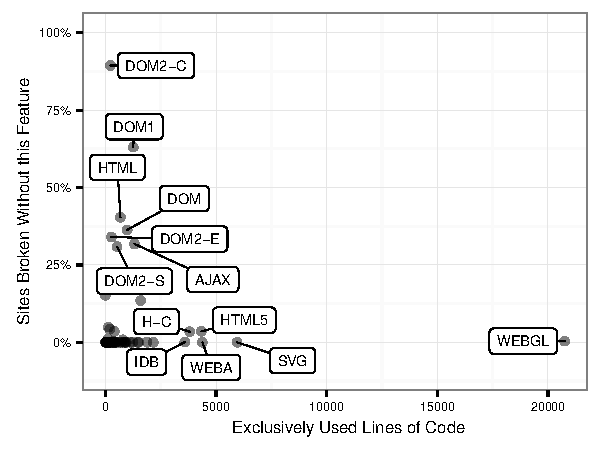
\includegraphics[width=.5\textwidth]{figures/loc_breakrate.pdf}
  \caption{A scatter plot showing the LOC measured to implement each standard, by how many sites in the Alexa 10k break when the standard is removed.}
  \label{fig:loc-breakrate}
\end{figure}

The amount of complexity each standard added to the browser code base varied
widely. \ref{fig:loc-breakrate} presents a comparison of each standard's
benefit (measured by the number of sites that require the standard to function)
against and number of lines of code uniquely needed to implement the standard,
using the method described in Section~\ref{cost-benefit:results:costs-loc}.

Points in the upper-left of \ref{fig:loc-breakrate} depict standards that are
frequently needed on the web, but which have relatively non-complex
implementations.  One example of such a standard is the \textit{DOM-Level 2
Core} standard, denoted by \textbf{DOM2-C}.  This standard extends
the browser's basic document modification methods.  This standard is needed for
89\% of websites to function correctly, suggesting it is highly beneficial to
web users.  The standard comes with a low security cost; our technique
identifies only 225 lines of code that are only included to enable this
standard (most of the code that implements this standard is shared by the
implementations of other standards).

Points in the lower-right of the figure depict standards that provide
little benefit, but which are responsible for a great deal
of complexity in the browser's code base.  The \textit{Scalable Vector
Graphics} standard, denoted by \textbf{SVG}, is an example of
such a high-cost, low-benefit standard.  The standard allows website authors to
dynamically create and interact with embedded \gls{svg} documents through \JS.
The standard is required for core functionality in approximately 0\% of
websites on the \ATK, while adding a large amount of complexity to the
browser's code base (at least 5,949 exclusive lines of code, more than our
technique identified for any other standard).


\subsection{Threats to Validity}
The main threat to validity in these measurements is the accuracy of our
human-executed casual browsing scenario. Regarding internal validity, the high
agreement between the two site-measuring workers suggests that our technique
was constant and replicable.  The students who worked on this project spent
over 500 hours combined performing these casual browsing tasks and recording
their results, and while they were completely separated while actively
browsing, they spent a good deal of time comparing notes about how to fully
exercise the functionality of a website within the 70 second time window for
each site.

External validity, the extent to which our results can be generalized, is also
a concern. Visiting a website for 70 or fewer seconds encapsulates 80\% of all
web page visits according to~\cite{liu2010understanding}, thus accurately
representing a majority of web browsing activity, especially when visiting
untrusted websites. Furthermore, while our experiment does not evaluate
functionality that is only available to authenticated users, we believe that
protection against unknown sites---the content aggregators, pop-up ads, or
occasionally consulted websites that a user does not interact with enough to
trust---are precisely the sites that deserve the most caution.
